
\subsection{Existing Technology}
A survey into how technology can support habit formation and behaviour change~\cite{survey_on_current_apps_of_steel}, reports a large number of habit forming systems are mobile apps. Studies into the effectiveness of these apps has been recently conducted~\cite{article_beyond_self_tracking_designing_apps, article_dont_kick_habit} revealing that although most of these apps are rated highly, they do not ground themselves in behaviour change theory. Further surveys of these apps~\cite{survey_on_apps_2} suggest that habit performance is not sustained when the app is removed, due to the lack of habit automaticity built during the habit tracking process. Using apps consistently to manage behaviour can create a notable difference in the person when the system is removed~\cite{article_my_phone_is_part_of_my_soul}.
This is also the case with many behaviour change systems, when the system is removed any improved performance is lost~\cite{article_dont_kick_habit, article_realtime_feedback_improving_medication_taking}. Building habit automaticity requires the desired action to be built around an existing routine~\cite{article_how_habits_formed_modelling_habit_formation, article_implementation_intentions_multicue}. Technology should help with routine creation by having additional checks to guard against changes in routine that remind people about their habit if their situation changes and issue post-completion notifications to check if the action has already happened~\cite{article_dont_forget_your_pill}. This is vital for sustaining performance and building habit automaticity.

\subsubsection*{Choice of System}
Although there has been lots of research using mobile apps for behaviour change interventions~\cite{survey_on_current_apps_of_steel} (Figure~\ref{fig:prototype_table}). There are plenty of other options available when designing be behaviour change interventions. One option that has been recently used for behaviour change interventions are \textit{chatbots}. They have been integrated into messaging apps, such as the \textit{Telegram} app to track food habits~\cite{telegram_bot_tracking_habits} and are seen as the next big thing in HCI~\cite{chatbots_and_new_world_of_hci}. Chatbots are applications that parse questions using Natural Language Processing (NLP) to provide a response and are platform independent. This means the bot can be accessed on mobile phones and desktops. Bots act as a user interface to expose data and would use online services to parse the response, such as Amazon lex (\url{https://aws.amazon.com/lex/}). These programs have conversations with users to achieve a goal and are not new inventions. Since 1966~\cite{article_eliza}, Eliza by Weizenbaum, used simple expression matching to return a certain response for user trials. In the present day, these applications (referred to as both bots and chatbots), are found integrated into many different apps on the majority of users mobile phones. For example, \textit{Facebook Messenger} (\url{www.messenger.com}), a popular messaging application encourages developers to create bots to interact with their users. These bots act as a real person with similar interaction flow, plus a few additional features, such as \textit{Quick Replies}~\cite{doc_fb_quick_replies} for revealing a list of options to a user. Quick Replies provide a way to present buttons to the user in response to a message (Figure~\ref{fig:healthy_bot_and_poncho}). However, these bots would not reply like a real person, but rather would only reply if that question was pre-trained using machine learning algorithms. This technology requires the bot to be trained on a large set of data and the majority of use cases would have to be accounted for. Natural language processing would enable users to chat to the bot and get a friendly understandable reply. However, this interaction may build a dependence on the user-chatbot interaction and could lead to losing automaticity.

\renewcommand{\arraystretch}{1.5} % Increase line height of the following tables
\begin{figure}[H] % ht
\begin{center}
\begin{tabular}{ |p{3.8cm}|p{2.5cm}|p{4cm}|p{2.5cm}|p{2cm}| }
 \hline
 \textbf{} & \textbf{Mobile App} & \textbf{Cross-Platform App} & \textbf{Webapp} & \textbf{Chatbot} \\ \hline
 Notifications & \cmark & \cmark & \xmark & \cmark \\ \hline
 Development Time & Long & Medium & Short & Short \\ \hline
 High Availability & \xmark & \xmark & \cmark & \cmark \\ \hline
 Simplicity & \xmark & \xmark & \cmark & \cmark \\
 \hline
\end{tabular}
\end{center}
    \caption{Comparing different options for behaviour change interventions.}
    \label{fig:prototype_table}
\end{figure}

Another design option is building a \textit{webapp}. However, the functionality is limited, due to the lack of the notification feature in current webapps. To allow notifications the webapp could be paired with another native app or use SMS (Short Message Service) notifications. However, because these technologies are separated it is more difficult to get users to respond and install a separate app. Another design option is a native mobile app as has the ability to supply notifications, but for each platform a completely separate app would need to be built and users would need to download the app before it would be available to them. A single cross-platform app could be constructed to reduce development time and complexity, but still users would need to download the app to start using it. A webapp has the advantage of being available to all users with a web browser (with users being able to save the site to home screen), but without notifications on all platforms (iOS only), it won't meet our requirements. Finally, a chatbot integrated into a popular messaging platform is easily available (if you have the messaging app already installed), simple (the user interface is already supplied), works on any platform the messaging app is available on and has notifications built in. The table (Figure~\ref{fig:prototype_table}) summarises the available development choices for a system that meets our aim.

\subsection{Platform}
The platform for the tool needed to be highly available for participants, interactive and time effective to build.
A chatbot provides us access to both the mobile platform and the desktop platform, granting us access to a highly available, contextually aware and interactive platform~\cite{article_my_phone_is_part_of_my_soul, article_mhealth}.

There are lots of options about what platform to build the chatbot into (Figure~\ref{fig:chatbot_platform_table}). For example, \textit{Slack} (\url{www.slack.com}) bots (Figure~\ref{fig:healthy_bot_and_poncho}) provide additional functionality to the popular workplace communication service and can complete complex tasks such as habit tracking (\url{https://healthybot.io}). \textit{Whatsapp} (\url{www.whatsapp.com}) also provides interactive features with a large user base, however it lacks many additional features, such as quick replies. \textit{Telegram} (\url{www.telegram.org}) and \textit{Facebook Messenger} (\url{www.messenger.com}) have these additional features, but only Facebook Messenger has the large user base. Therefore, because our main aim is to interact with lots of people easily, we need to target existing platforms that have high participant availability.

\begin{figure}[H] % ht
\begin{center}
\begin{tabular}{ |p{3.8cm}|p{4cm}|p{2.2cm}|p{1cm}|p{1.8cm}|p{1.3cm}| }
 \hline
 \textbf{} & \textbf{Facebook Messenger} & \textbf{WhatsApp} & \textbf{SMS} & \textbf{Telegram} & \textbf{Slack} \\ \hline
 High Availability & \cmark & \cmark & \cmark & \xmark & \xmark \\ \hline
 Interactive & \cmark & \cmark & \xmark & \cmark & \cmark \\ \hline
 Additional Features & \cmark & \xmark & \xmark & \cmark & \cmark \\
 \hline
\end{tabular}
\end{center}
    \caption{Comparing different chatbot platforms.}
    \label{fig:chatbot_platform_table}

\end{figure}


Facebook Messenger looks like the attractive option for user interaction with the ease of additional features, such as quick replies and with the benefit of:

\begin{itemize}
  \item 1,200 Million active users per month (as of April 2017)~\cite{fb_messenger_stats}
  \item Embedded into a service users already use
  \item Quick replies allows for easy interaction
\end{itemize}

The success of the chatbot will depend on how people differentiate between the bot and another contact and if people prefer the interaction.

\begin{figure}[H]
  \centering
  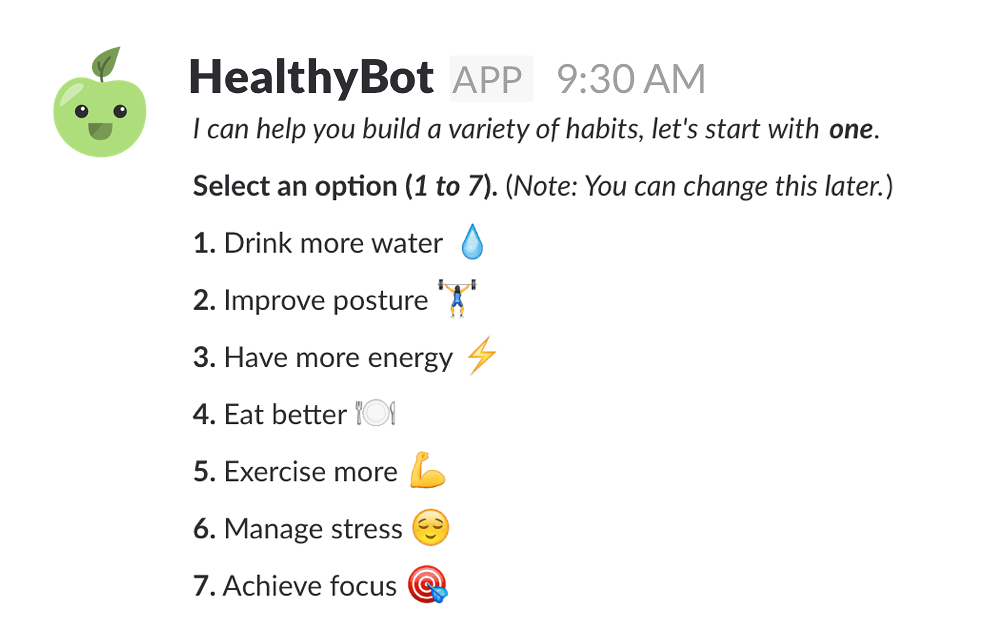
\includegraphics[width=3in]{../resources/existing-bots/healthy-bot.png}
  \hspace{10px}
  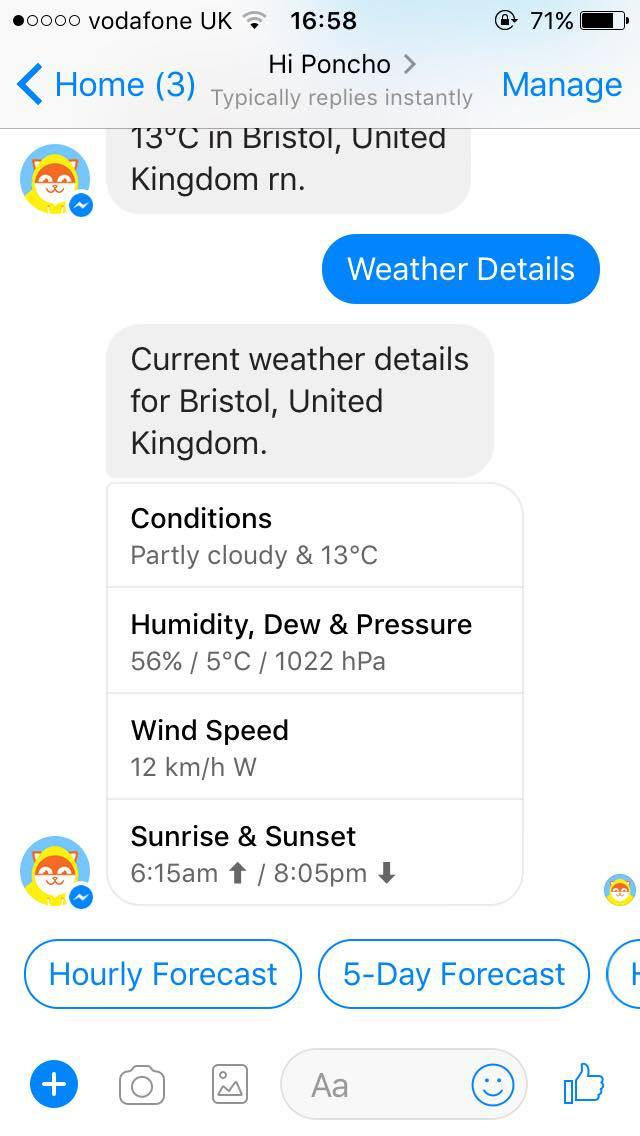
\includegraphics[width=1.7in]{../resources/existing-bots/poncho.jpg}
  \caption{Left: \textit{Healthy Bot}: a Slack chatbot for forming new positive habits. Right: \textit{Poncho}: an example of Facebook Messenger Weather Chatbot.}
  \label{fig:healthy_bot_and_poncho}
\end{figure}

\subsection*{Facebook Messenger}
Interaction with existing Facebook Messenger chatbots is varied. Existing bots use three methods of interaction that utilise different areas of the Facebook Messenger interface. The first method fully utilises natural language processing. The bot sits patiently until it receives a message, then it sends the message off to a service that performs processing and returns the message breakdown. The bot then chooses an action based on the message. For example, the Poncho weather bot (\url{https://poncho.is/}) displays the forecast for Bristol if you message \textit{bristol forecast}. As previously discussed this method of interaction does not suit our needs because we do not require users to ask questions to the bot.

\begin{figure}[H]
  \centering
  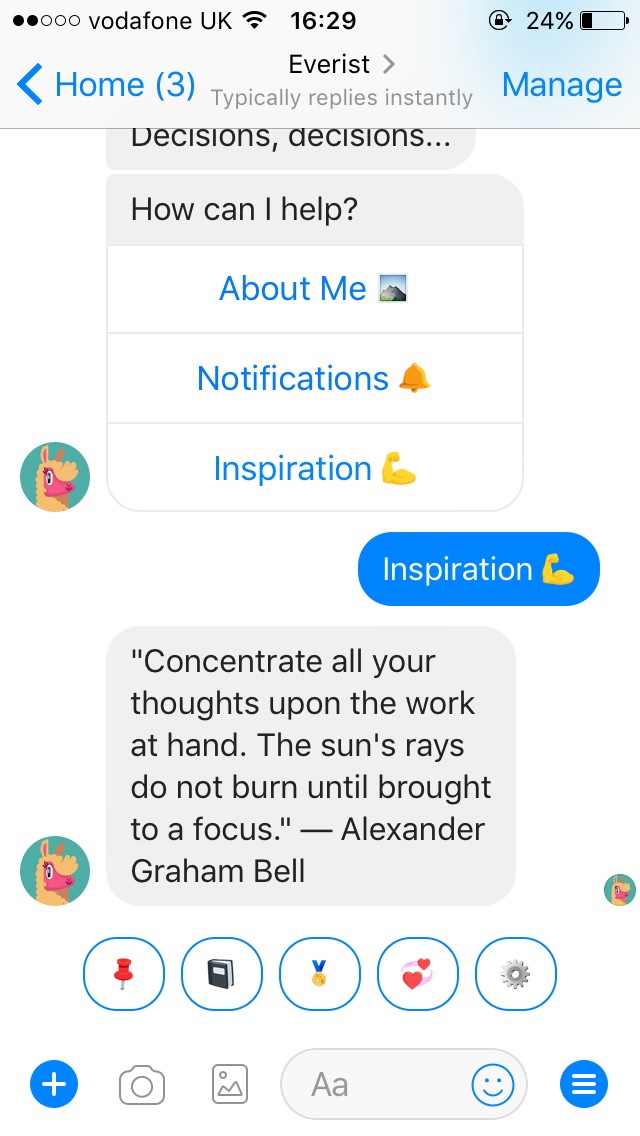
\includegraphics[width=1.9in]{../resources/existing-bots/everist.png}
  \hspace{10px}
  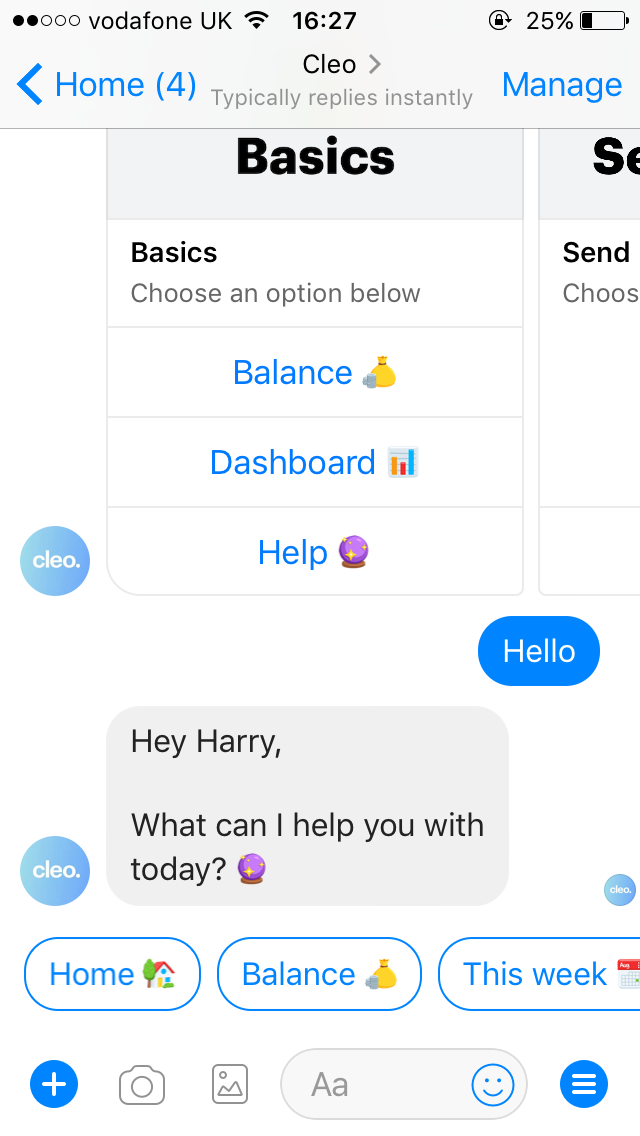
\includegraphics[width=1.9in]{../resources/existing-bots/cleo.png}
  \hspace{10px}
  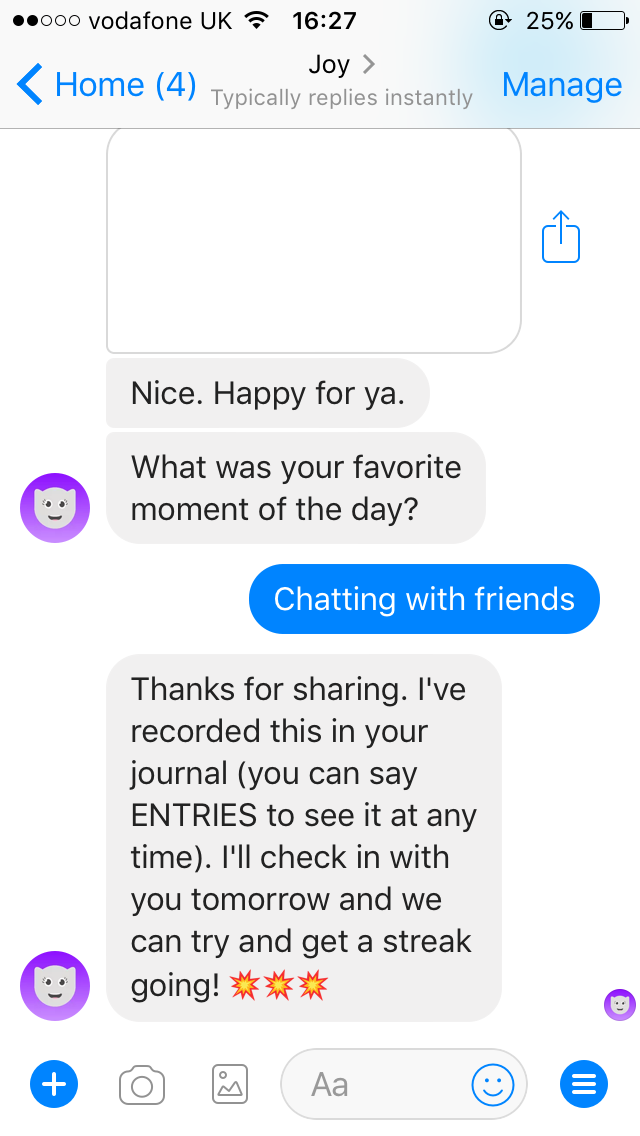
\includegraphics[width=1.9in]{../resources/existing-bots/joy-ai.png}
  \caption{Examples of existing chatbots that help track and form new habits with different methods of user interaction. Left Everist (\url{https://www.everist.ai/}), middle Cleo (\url{https://meetcleo.com/}), right Joy (\url{http://www.hellojoy.ai/}).}
  \label{fig:chatbots_examples}
\end{figure}


The second method does not use natural language processing and quick replies are heavily utilised. Everist and Cleo bots (Figure~\ref{fig:chatbots_examples}) use quick replies almost like a menu with a set of options. After users message the bot once, the set of quick replies are returned to encourage users to only use these as the method of communication. Although this makes coding the prototype easier, it is difficult to get \textit{free text} from users. Finally, Joy (Figure~\ref{fig:chatbots_examples}) uses a combination of free text and quick replies to set-up users and interact with them every day. This is the combination that Harry's Habits will use to get free text from users and enable quick choice from a menu of actions.


\subsubsection*{Supporting Habit Formation}
Harry's Habits will be built Facebook Messenger --- an existing social network that people are used to --- to track habits and deliver rewards. The social scaffolding around the interaction and the integration with the platform will mean that interactions with the bot will be visible alongside participant's other conversations, making it easier to report the completion of the habit~\cite{the_power_of_logging_mobile_notifications}. The bot will track simple actions of similar difficulty to reduce the amount of time needed before the action turns into a habit~\cite{article_how_habits_formed_modelling_habit_formation}. Other design methods to help people form new habits were looked at but will not be added to the prototype to limit the scope of the project. For example, gamification, such as using gambling elements and engineering luck into games have been shown to encourage interaction~\cite{article_free_to_play_making_money_from_games_you_give_away} and using monetary rewards to create a feedback loop where people keep coming back for the reward~\cite{website_how_to_design_feedback_loops}. Both of these elements can help with interaction but do not build habit automaticity, therefore leading to a drop in performance when the feedback is removed.

\subsection{Design Requirements} \label{recommendations}
After reviewing literature from habit formation, modality task performance and existing habit formation technology. A new set of design requirements is created, for building a chatbot that is grounded in habit formation theory and focused on rewards.

\textbf{REQ 1. Help users define a memorable strategy.}\newline
Help users make personalised routines and provide examples of existing strategies based on REQ 1, 2 from~\cite{article_beyond_self_tracking_designing_apps} and REQ 2, 4 from~\cite{article_taxonomy_motivational_affordances_meaningful}.

\textbf{REQ 2. Remind them about cues and remembering strategies.}\newline
Reminders can effectively support prospective memory in the short-term, increase the logging of health data~\cite{the_power_of_logging_mobile_notifications} and educate them about what they should perform in the long-term. Based on REQ 4 from~\cite{article_beyond_self_tracking_designing_apps} and REQ 3 from~\cite{article_taxonomy_motivational_affordances_meaningful}.

\textbf{REQ 3. Reward users.}\newline
Positive reinforcement rewards are a good form of external motivation. Based on REQ 4 from~\cite{article_taxonomy_motivational_affordances_meaningful}.

\textbf{REQ 4. Send positive reinforcement from different modes.}\newline
Task performance is impacted when sending positive reinforcement from visual, auditory and visual-auditory modalities.

\textbf{REQ 5. Check if the action has already happened.}\newline
People find it easy to forget whether an automatic task was completed. Therefore a post completion notification to check to see if the action has already happened should be issued, based on REQ 6 from~\cite{article_beyond_self_tracking_designing_apps} and REQ 1 from~\cite{article_taxonomy_motivational_affordances_meaningful}.

\textbf{REQ 6. Disable cue reminders when behaviour is routine.}\newline
Relying on reminders in the long-term can hinder habit development, therefore ease off from reminders later. Based on REQ 5 from~\cite{article_beyond_self_tracking_designing_apps} and REQ 5 from~\cite{article_taxonomy_motivational_affordances_meaningful}.


\newpage
\section{Design}
A prototype was constructed to track habits and deliver rewards based on the requirements from Section~\ref{recommendations}.

\subsection*{Track Habits}
To help users define a memorable strategy (REQ 1) users are allowed to personalise the experience slightly with their own routine and choice of habit with examples given during the setup phase (Figure~\ref{fig:setup_flow_screenshots}). Post completion checks are delivered after users existing routine to check if the action has already happened (REQ 5) and remind users about their cue (REQ 2). Finally, positive reinforcement is delivered after the habit has been performed from a modality to improve habit performance (REQ 4).

\begin{figure}[H]
  \centering
  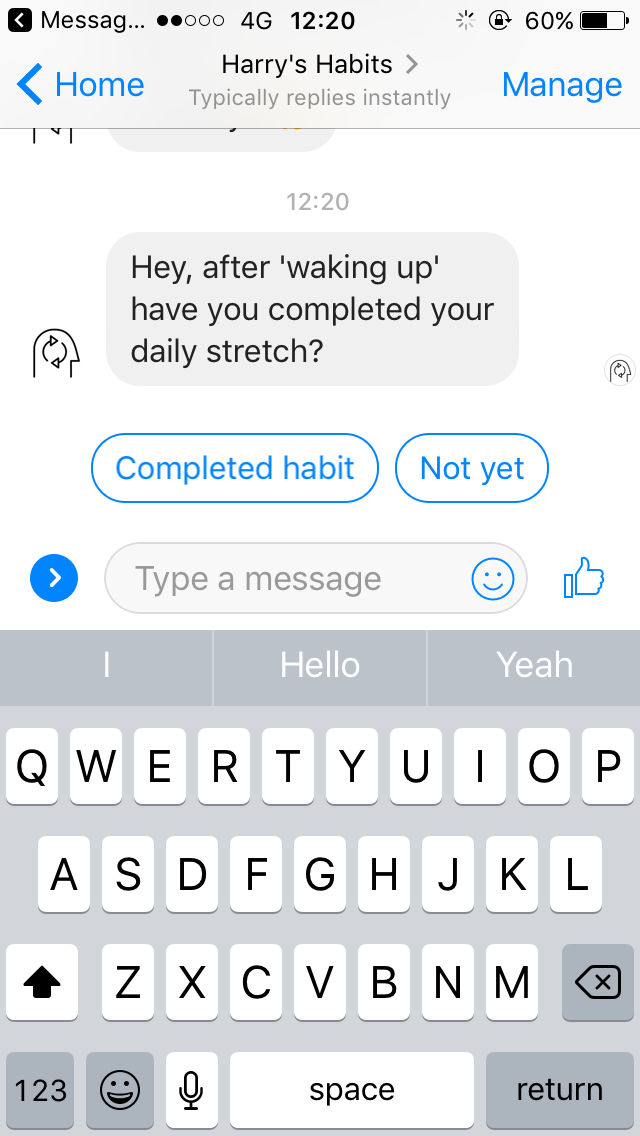
\includegraphics[width=1.5in]{resources/figures/reminder.png}
  \hspace{10px}
  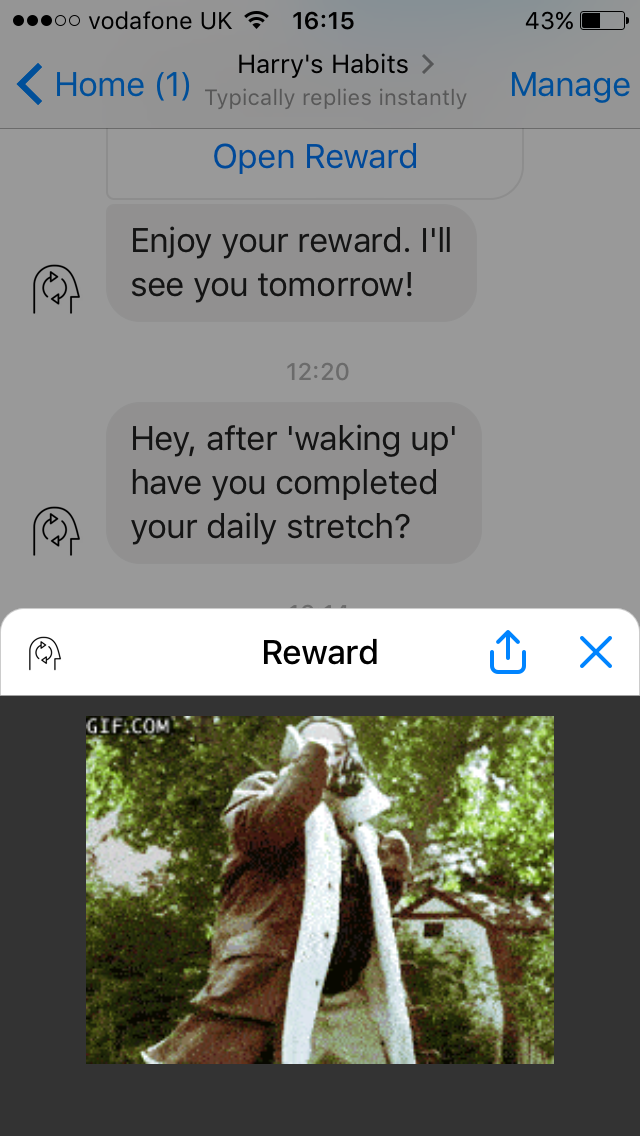
\includegraphics[width=1.5in]{resources/figures/reward-visual.png}
  \caption{Harry's Habits delivering a post completion message (left) and an example of a visual reward (right).}
  \label{fig:delivering_reward}
\end{figure}


\subsection*{Delivering Rewards}
To reward users (REQ 3) and to answer all research questions. Rewards from three different modalities are delivered by the bot: visual, auditory and visual-auditory. The content of these rewards are experimented with. For the visual rewards, popular internet memes are used, i.e. content that is passed along from person to person via social media posts~\cite{meme_definition}. Humorous GIF memes make people laugh and are popular on some social media sites where they usually are the most engaging content~\cite{meme_gifs_are_good}. Given that the bot is integrated with Facebook, and that Facebook introduced built-in support for animated GIFs~\cite{fb_gif_rollout}, memes will integrate well with the bot environment. These rewards are displayed to the user within the chatbot after they complete their habit (Figure~\ref{fig:delivering_reward}). The modalities are mapped to identify a pattern across the modes before they are implemented and adapted for delivering rewards. The rewards were aimed at motivating participants to keep coming back every day and completing their habits. Several GIFs and audio files were identified that categorised themselves as motivational and each GIF file was vaguely matched and tweaked to match the audio frequency. The relationship between the audio and visuals is inferred, therefore this mapping is \textit{semi-congruent}.

\begin{figure}[H]
  \centering
  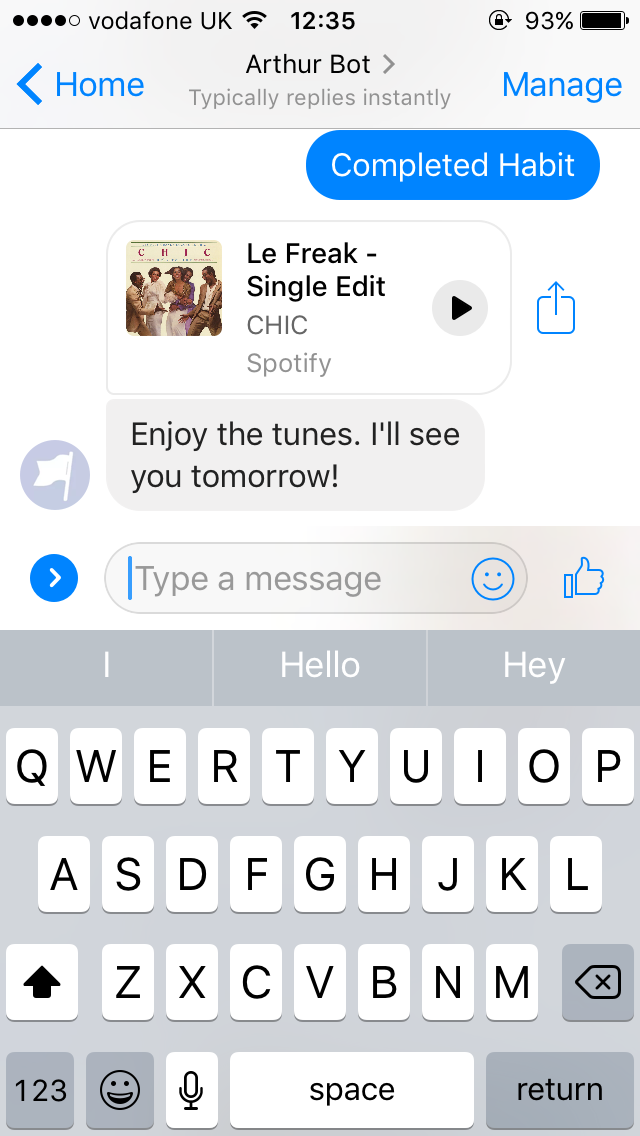
\includegraphics[width=1.5in]{../resources/design/reward-audio-inline.png}
  \hspace{10px}
  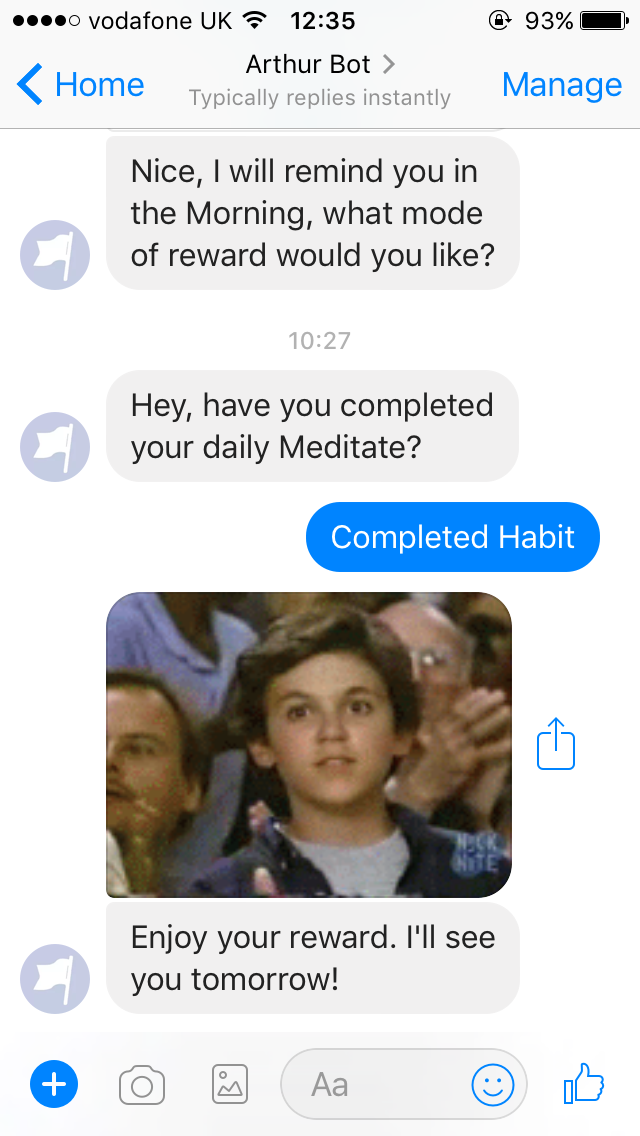
\includegraphics[width=1.5in]{../resources/design/reward-visual-inline.png}
  \caption{Inconsistent design with auditory and visual rewards when sent as a inline message.}
  \label{fig:rewards_inline}
\end{figure}

\subsection*{Design Interface Consistency}
During the design phase two different interface methods are discovered for delivering visual, auditory and visual-auditory rewards to users. First, GIFs and audio sent as a inline message to the user (Figure~\ref{fig:rewards_inline}). Second, a consistent method displays the reward from a website and links it to users (Figure~\ref{fig:rewards_consistency}). The first method (inline message) has the benefit of being native to Messenger, providing a better user experience, is faster to receive and requires less buttons to be pressed. However, each reward is not displayed consistently. Visual rewards started as soon as they were delivered, but the auditory reward had to have a \textit{play} button that had to be pressed before the audio started and the visual-auditory rewards also had a button that needed to be pressed. Inconsistency with delivery would make it difficult to evaluate the effectiveness of each reward. Therefore the second method is chosen (Figure~\ref{fig:rewards_consistency}) to allow for consistency when delivering rewards.


\begin{figure}[H]
  \centering
  \includegraphics[width=1.5in]{../resources/design/reward-visual-2.png}
  \hspace{10px}
  \includegraphics[width=1.5in]{../resources/design/reward-audio.png}
  \hspace{10px}
  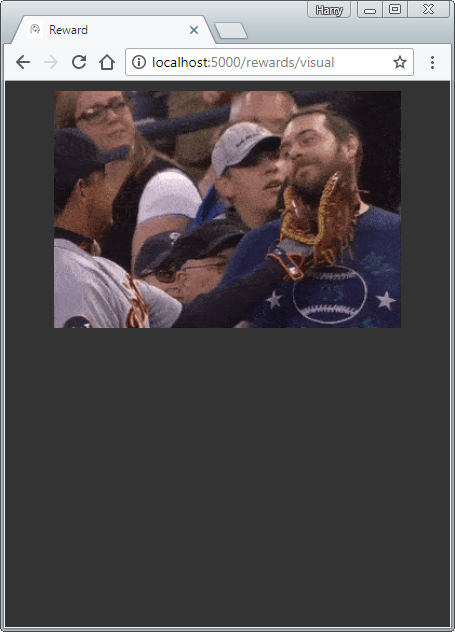
\includegraphics[width=1.7in]{../resources/design/reward-desktop-visual.png}
  \caption{Consistency between every type of reward modality on all platforms, displayed by a website. Left, iOS, visual reward. Middle, Android, auditory reward. Right, browser, visual-auditory reward.}
  \label{fig:rewards_consistency}
\end{figure}

\subsection{User Flows} \label{user_flow}
Full user interaction from setup to completing a reward was designed. The setup used a combination of quick replies and free text to gather demographic information and complete the setup for each user.

\begin{figure}[H]
  \centering
  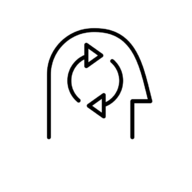
\includegraphics[width=1in]{../resources/logo.png}
  \caption{Harry's Habits logo was design by the Noun Project by Yu luck (\url{https://thenounproject.com/term/custom/402041/}).}
  \label{fig:logo}
\end{figure}


\subsubsection{Setup Flow} \label{setup_flow}

\begin{itemize}
  \item Press button that opens the bot in the Facebook Messenger app.
  \item Answer a series of setup questions to the bot via the Facebook Messenger app.
  \item User chooses an existing habit they would like to develop from a list.
  \item User supplies an existing routine to integrate their new habit into.
  \item User chooses a time the existing routine normally happens.
  \item User finishes the setup and closes the Facebook Messenger app.
\end{itemize}

\begin{figure}[H]
  \centering
  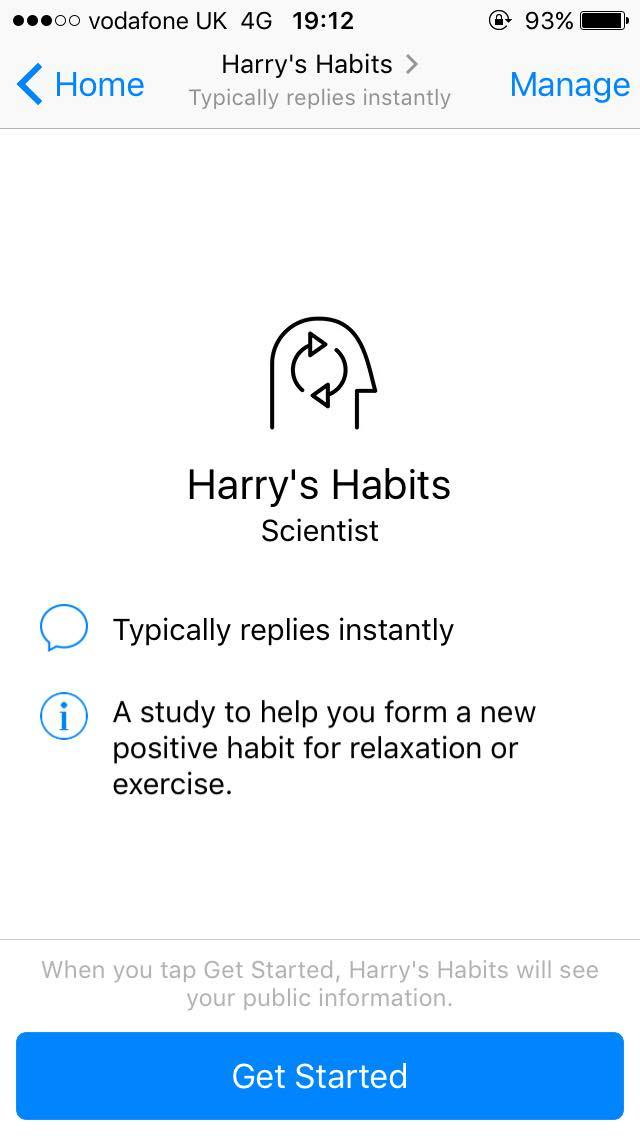
\includegraphics[width=1.4in]{resources/design/process/1.jpg}
  \hspace{10px}
  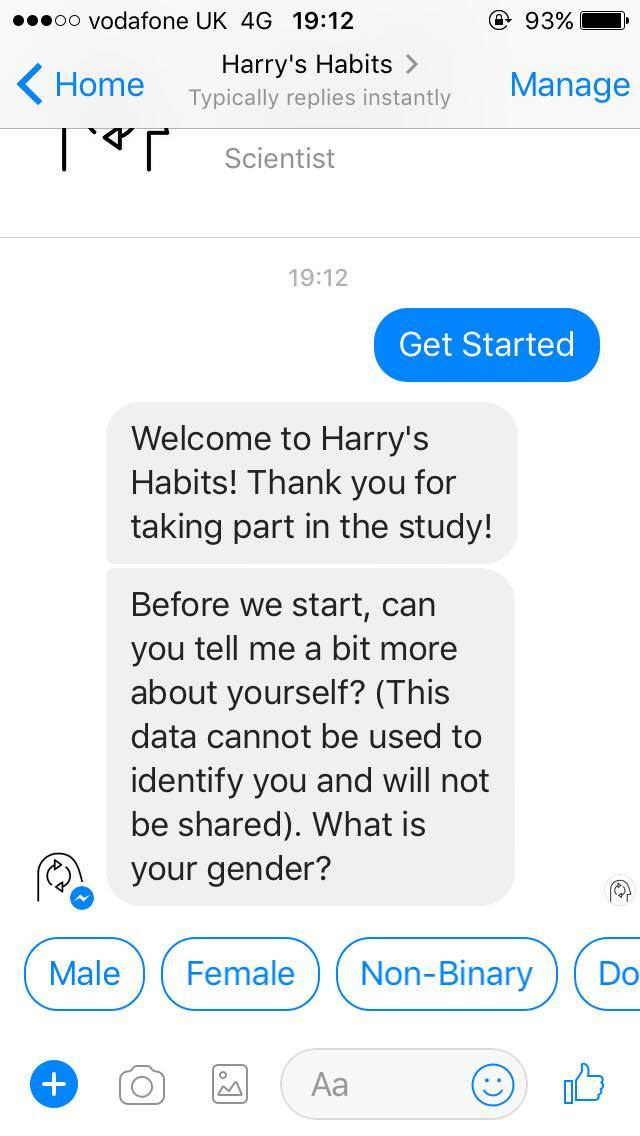
\includegraphics[width=1.4in]{resources/design/process/2.jpg}
  \hspace{10px}
  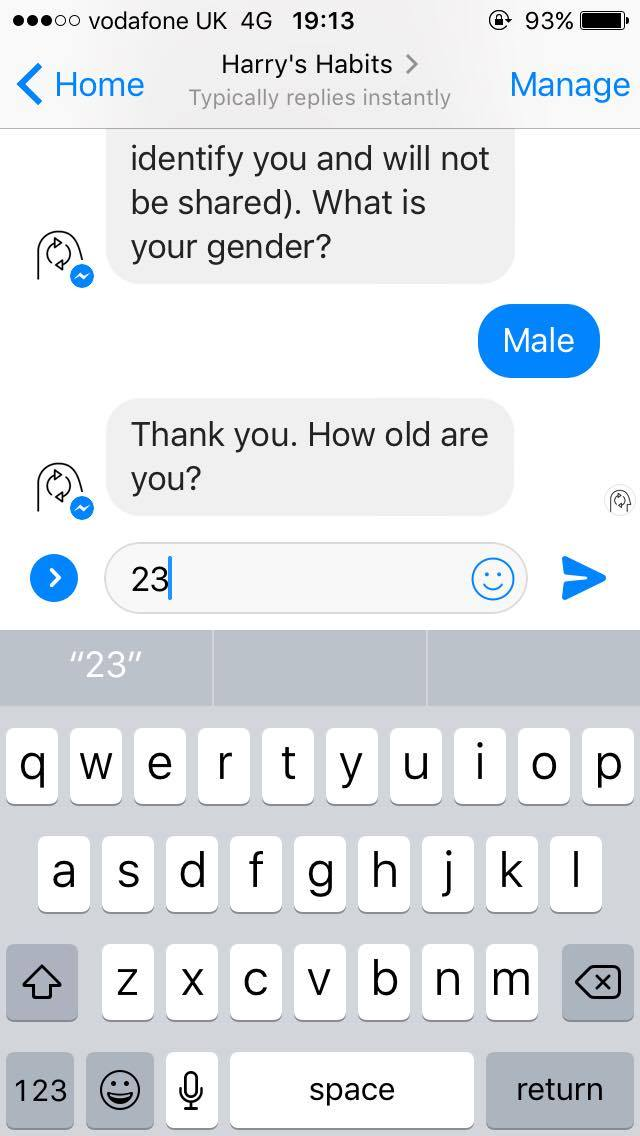
\includegraphics[width=1.4in]{resources/design/process/3.jpg}
  \hspace{10px}
  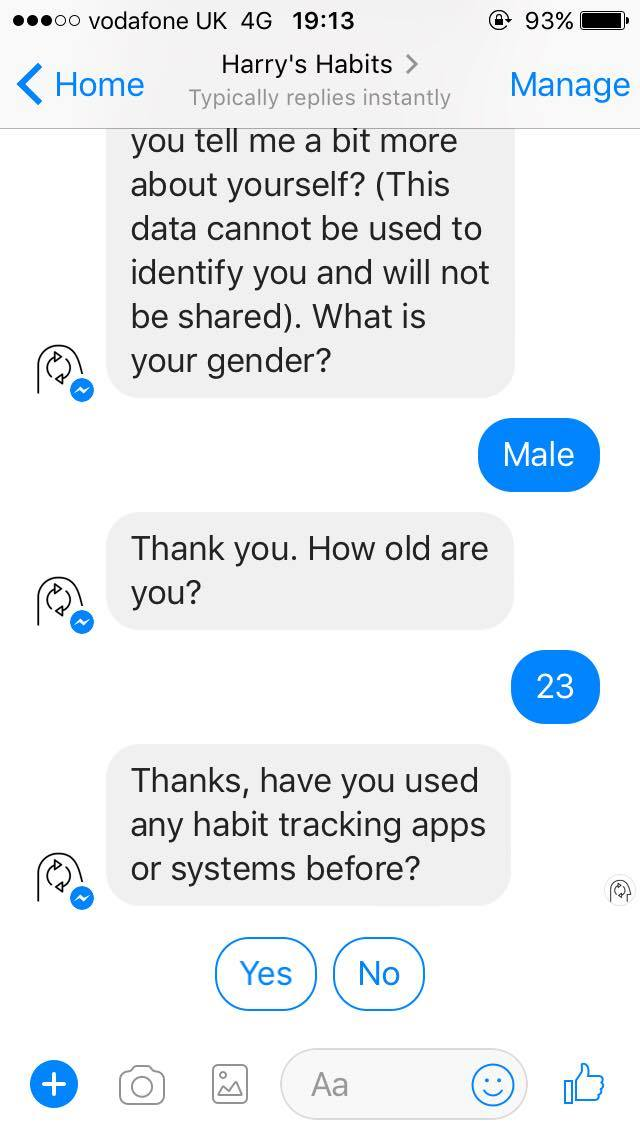
\includegraphics[width=1.4in]{resources/design/process/4.jpg}
  \newline
  \newline
  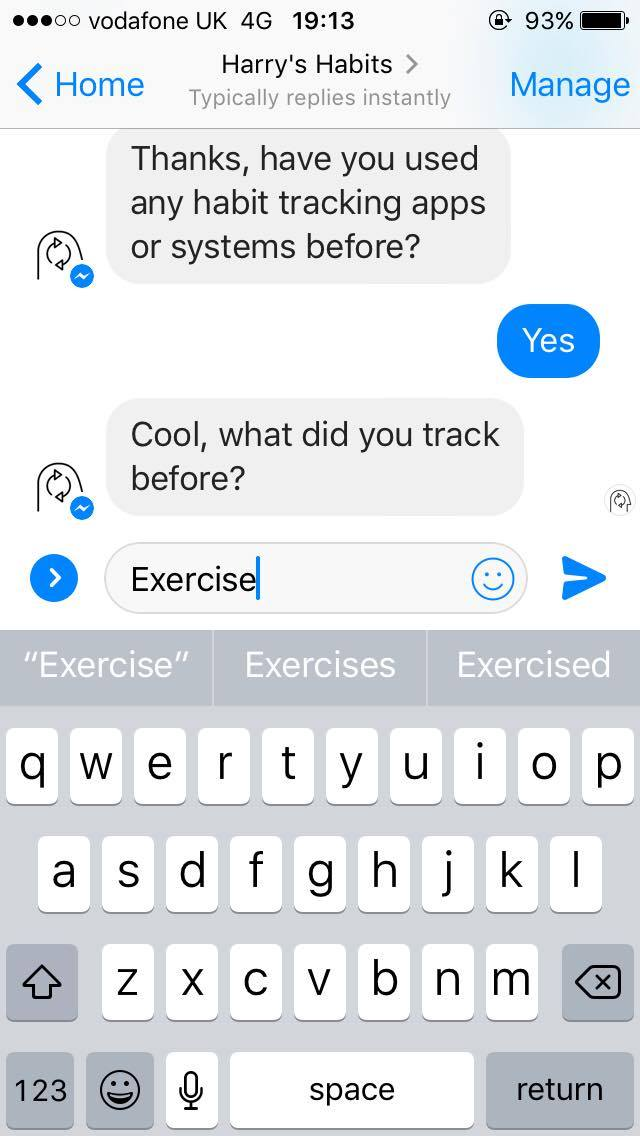
\includegraphics[width=1.4in]{resources/design/process/5.jpg}
  \hspace{10px}
  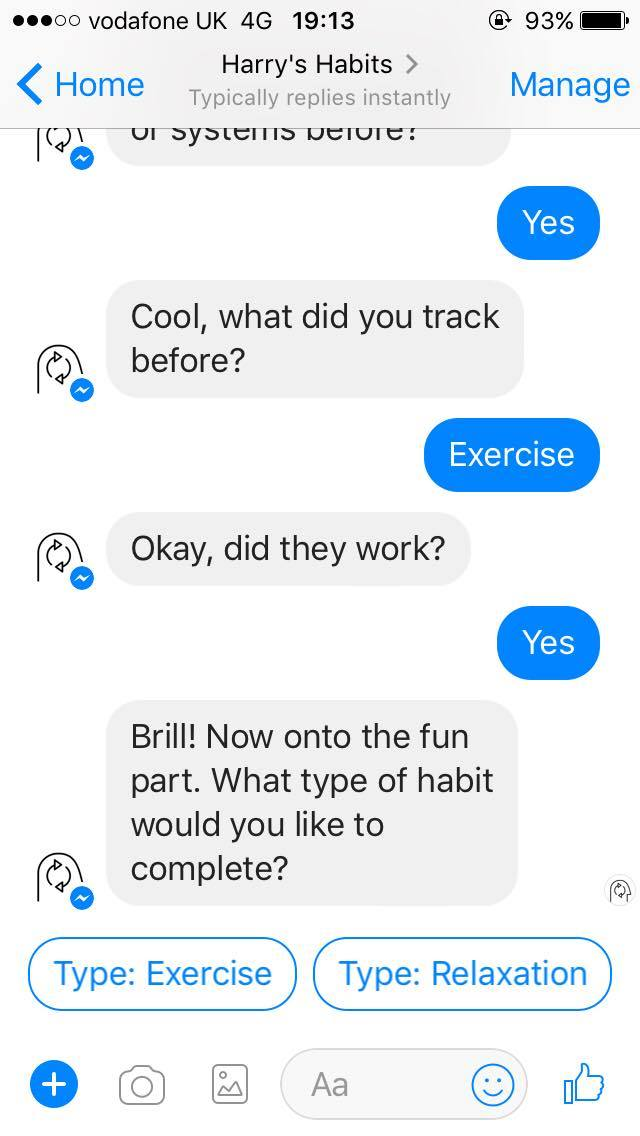
\includegraphics[width=1.4in]{resources/design/process/6.jpg}
  \hspace{10px}
  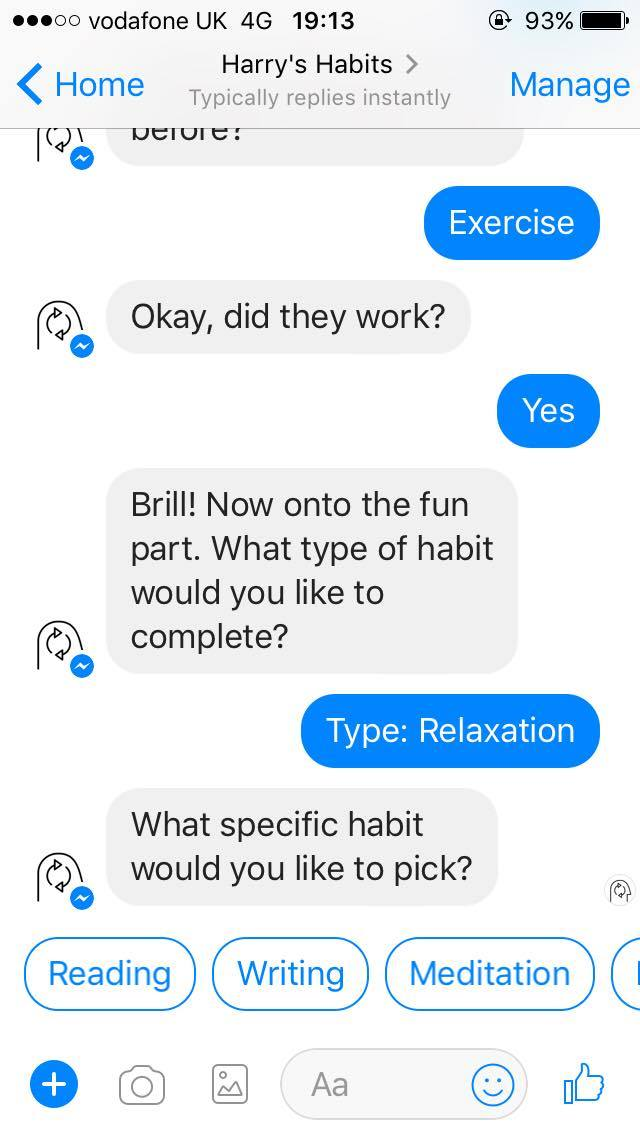
\includegraphics[width=1.4in]{resources/design/process/7.jpg}
  \hspace{10px}
  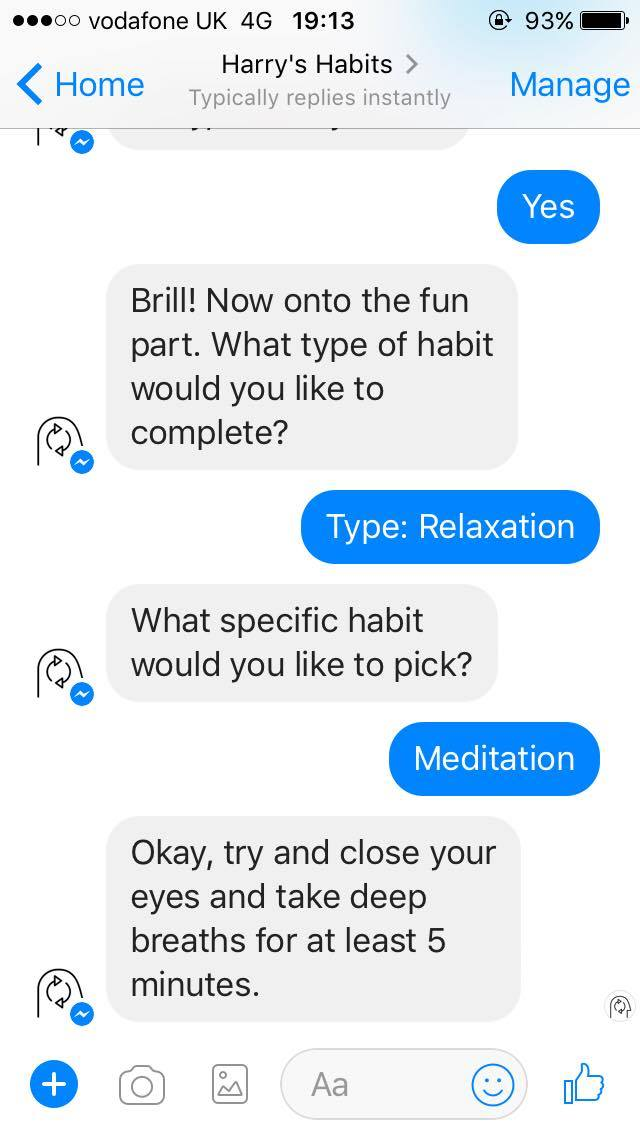
\includegraphics[width=1.4in]{resources/design/process/8.jpg}
  \newline
  \newline
  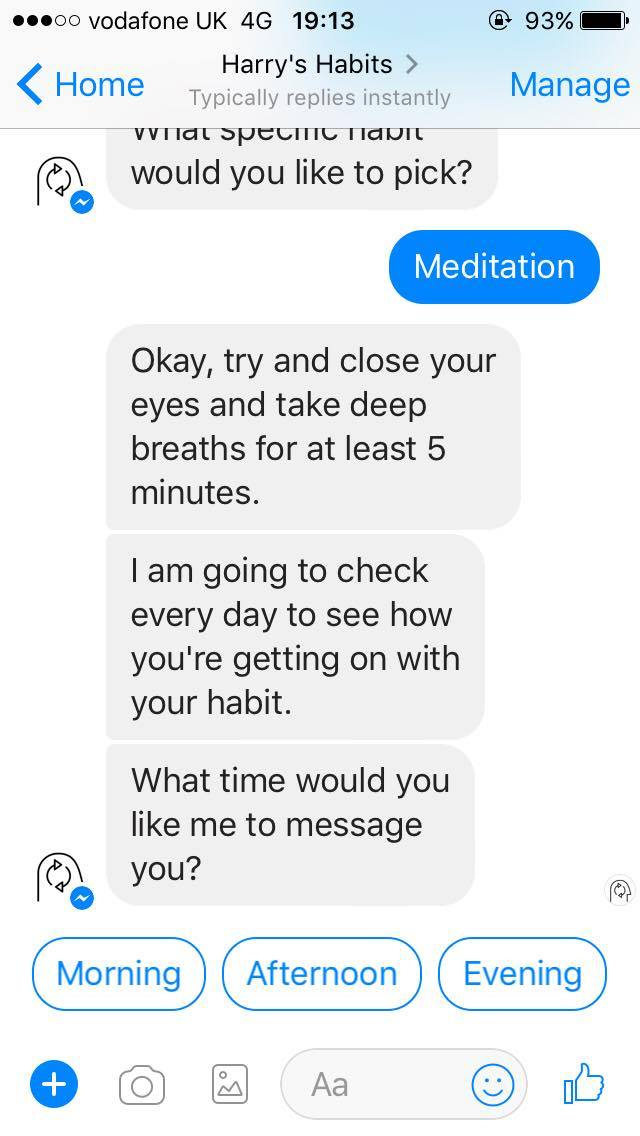
\includegraphics[width=1.4in]{resources/design/process/9.jpg}
  \hspace{10px}
  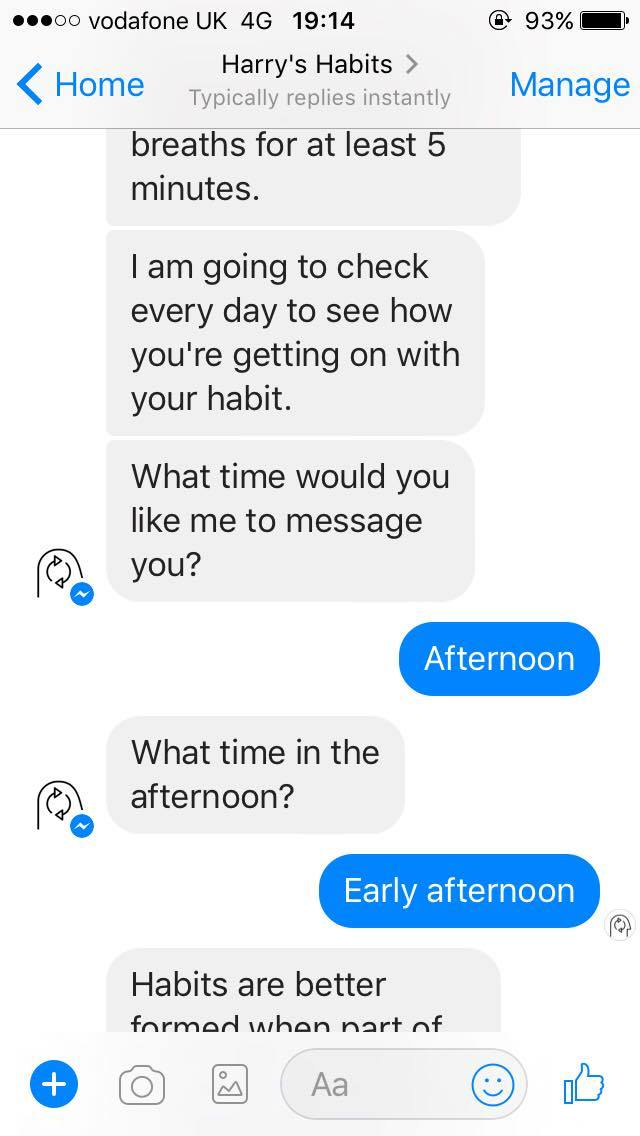
\includegraphics[width=1.4in]{resources/design/process/10.jpg}
  \hspace{10px}
  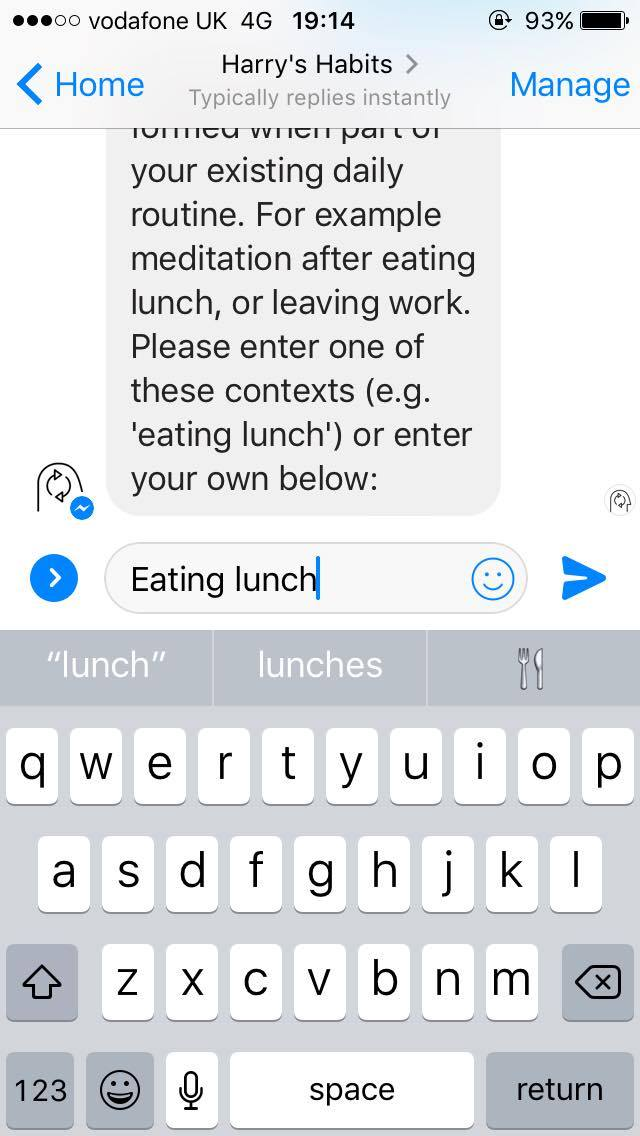
\includegraphics[width=1.4in]{resources/design/process/11.jpg}
  \hspace{10px}
  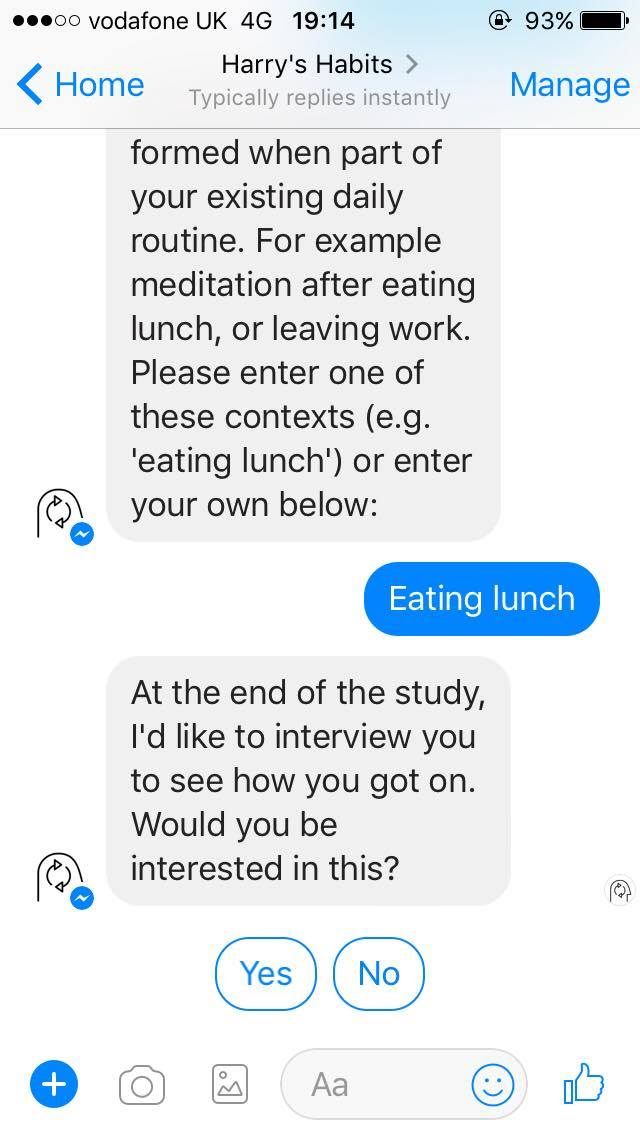
\includegraphics[width=1.4in]{resources/design/process/12.jpg}
  \caption{Setup flow for Harry's Habits.}
  \label{fig:setup_flow_screenshots}
\end{figure}

\begin{figure}[H]
  \centering
  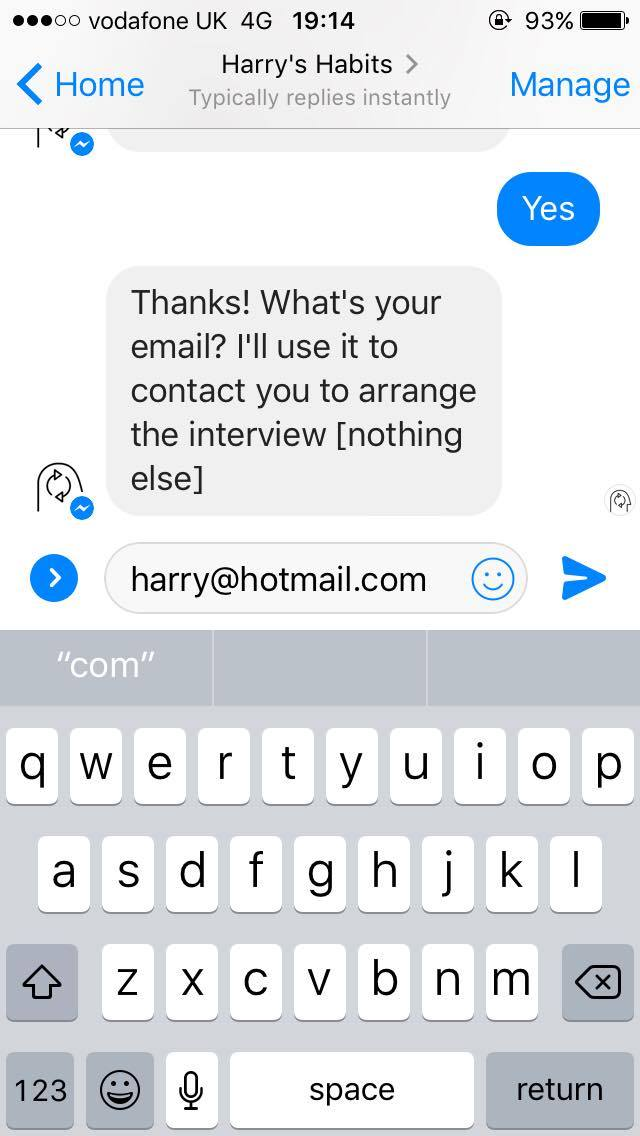
\includegraphics[width=1.5in]{resources/design/process/13.jpg}
  \hspace{10px}
  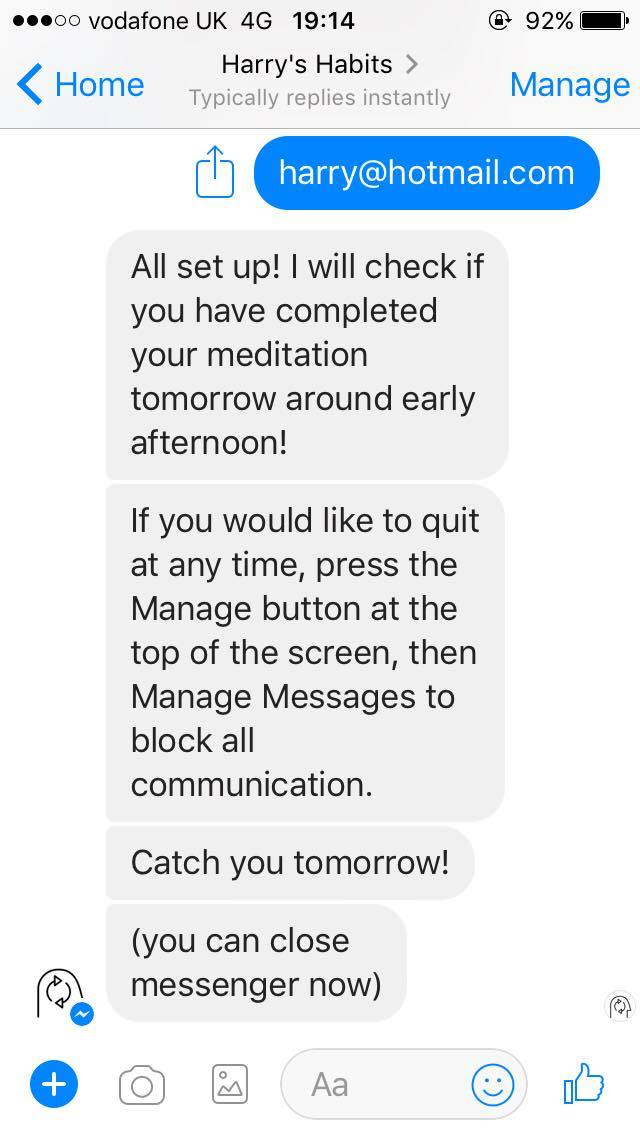
\includegraphics[width=1.5in]{resources/design/process/14.jpg}
  \hspace{10px}
  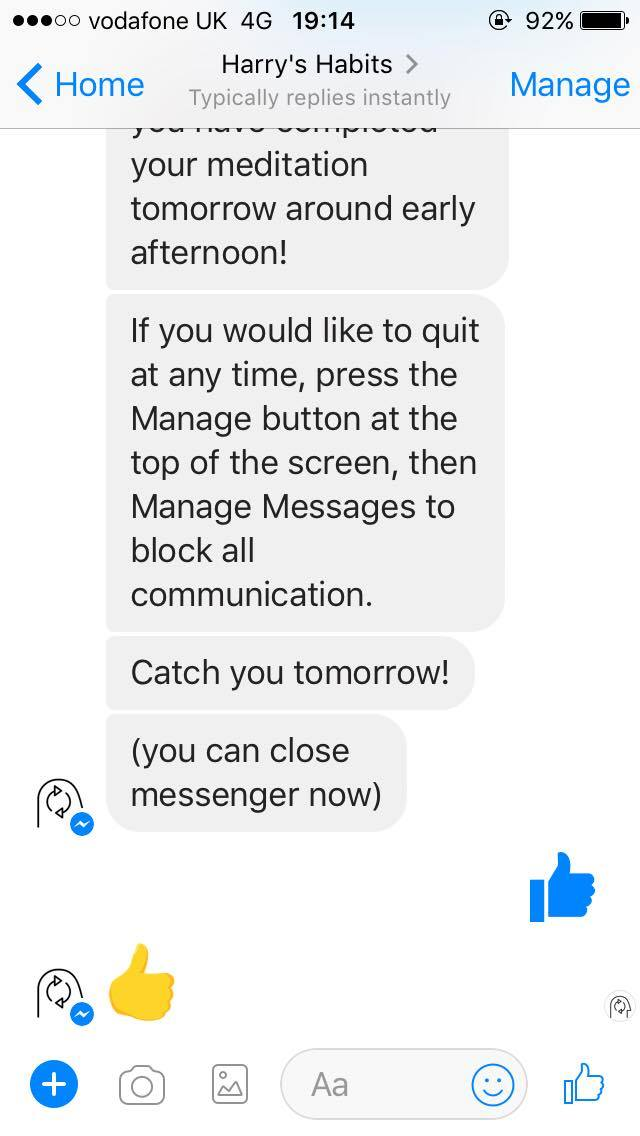
\includegraphics[width=1.5in]{resources/design/process/15.jpg}
  \caption{Continued: Setup flow for Harry's Habits.}
  \label{fig:setup_flow_screenshots_2}
\end{figure}



\subsubsection{Trigger Flow} \label{trigger_flow}
\begin{itemize}
  \item At the time of the existing routine the user performs their chosen habit.
  \item The user receives a notification after the routine, asking if they managed to complete their habit or if they need more time.
  \item If they need more time, the notification will \textit{snooze} for about an hour and be sent again.
  \item If users regularly snooze they will be asked if the time of their existing routine has changed.
  \item If users say they have completed their habit, they will be sent a quick reply message that links to a reward.
\end{itemize}

\begin{figure}[H]
  \centering
  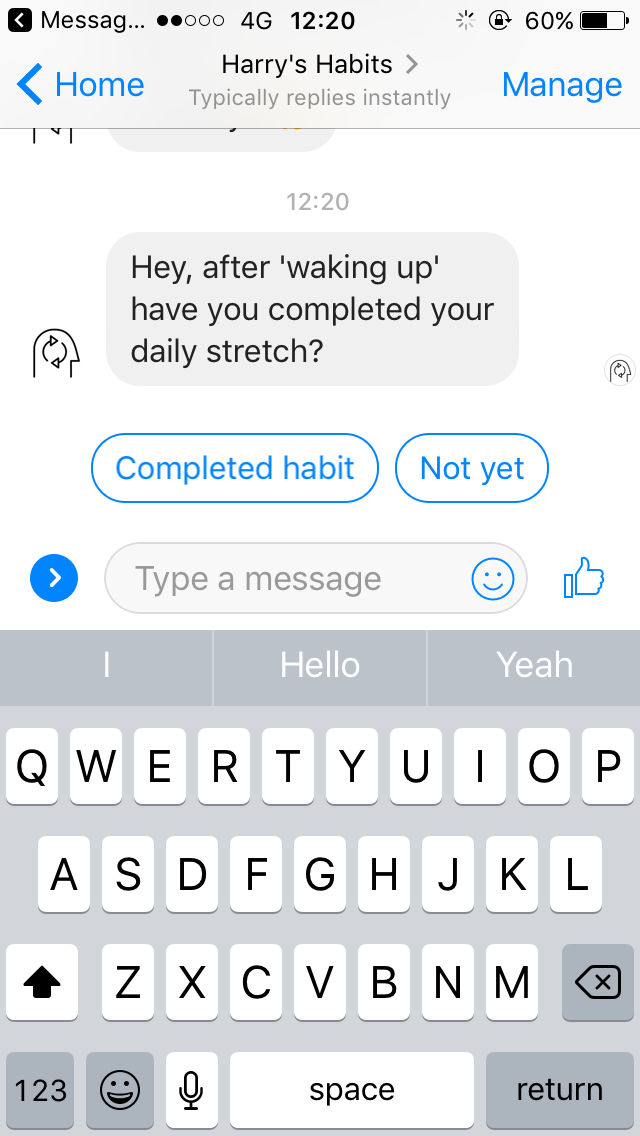
\includegraphics[width=2in]{resources/design/media/3.png}
  \hspace{10px}
  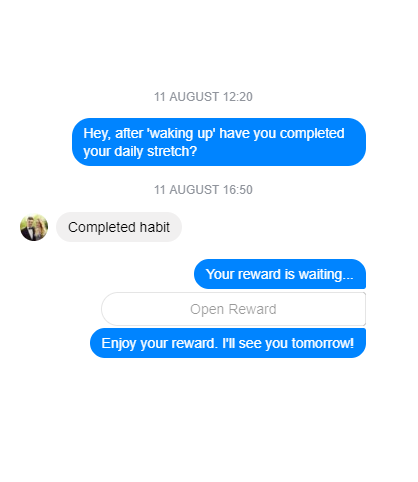
\includegraphics[width=2.8in]{resources/design/completed_habit.png}
  \caption{Trigger flow for Harry's Habits.}
  \label{fig:trigger_flow_screenshots}
\end{figure}


\subsubsection{Reward Flow} \label{reward_flow}


\begin{itemize}
  \item Users will press the reward button that will take them to a website that contains a link to open a reward. This allows the experience to be consistent for each reward modality.
  \item User will receive a reward from one of the following modalities:
  \begin{itemize}
    \item Visual: GIF with no audio
    \item Audio: soundtrack audio
    \item Visual-Auditory: GIF with soundtrack audio
  \end{itemize}
\end{itemize}

\begin{figure}[H]
  \centering
  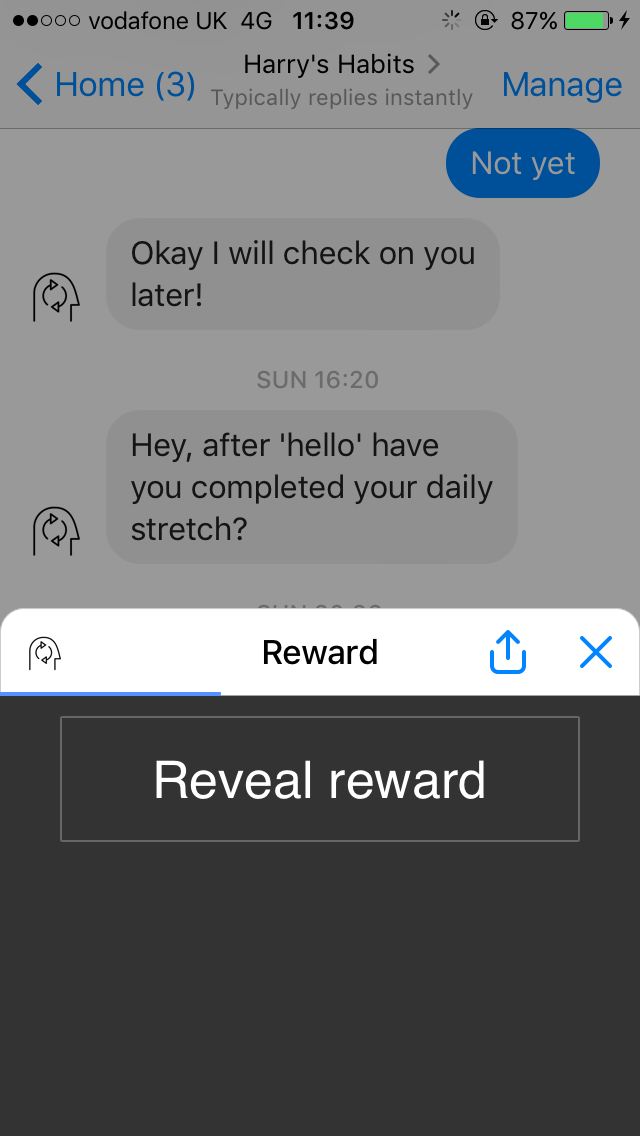
\includegraphics[width=1.8in]{resources/design/reward-visual-1.png}
\end{figure}
\begin{figure}[H]
  \centering
  \includegraphics[width=1.6in]{resources/design/reward-visual-2.png}
  \hspace{5px}
  \includegraphics[width=1.6in]{resources/design/reward-audio.png}
  \hspace{5px}
  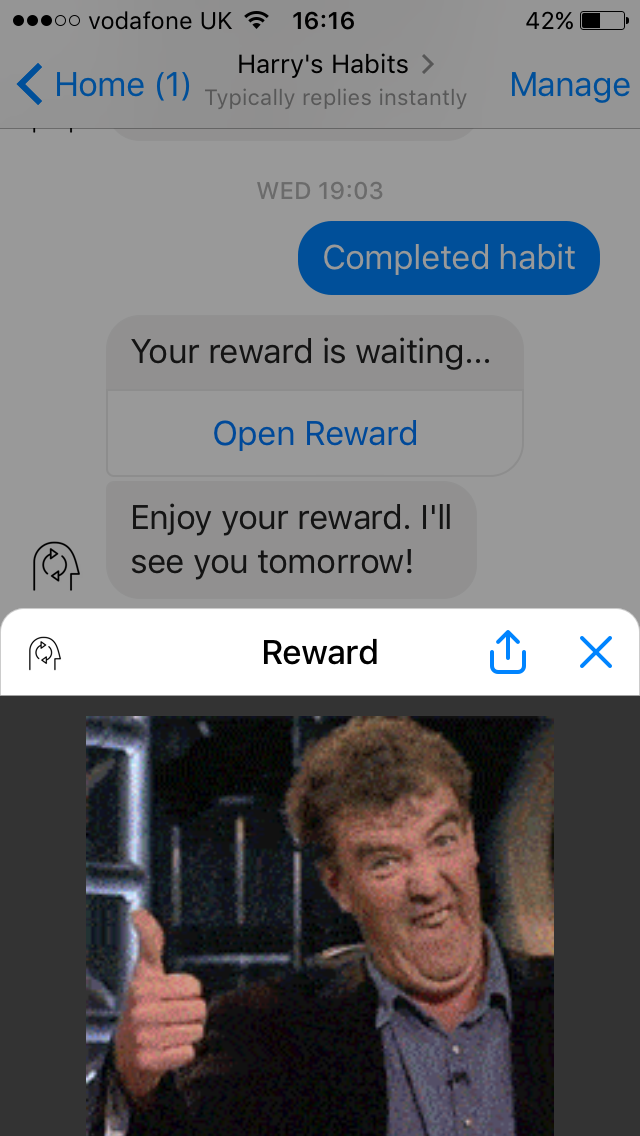
\includegraphics[width=1.6in]{resources/design/reward-visual-gif-2.png}
  \caption{Reward flow for visual, auditory and visual-auditory rewards for Harry's Habits.}
  \label{fig:reward_flow_screenshots}
\end{figure}

\newpage
